\documentclass[review]{elsarticle}

\usepackage{graphicx}
\usepackage[latin1]{inputenc}
\usepackage{pifont} 
\usepackage{import}
\usepackage{amsmath}
\usepackage{multirow}
\usepackage{graphicx,url}
\usepackage{placeins}
\usepackage{adjustbox}
\usepackage[english]{babel}
\usepackage{lipsum}
\usepackage{multicol}
\usepackage{textcomp}
\usepackage{listings}
\usepackage[svgnames]{xcolor} 
\usepackage{caption}
\usepackage{amsmath}
\usepackage{calc} 
\usepackage{array,url,kantlipsum}
\usepackage{algorithm}
\usepackage{algpseudocode}
\usepackage{lscape}
\usepackage{array}
\usepackage{longtable}
\usepackage{booktabs}
\usepackage{txfonts}
\usepackage{colortbl}%
  \newcommand{\myrowcolour}{\rowcolor[gray]{0.925}}
\newenvironment{Figure}
  {\par\medskip\noindent\minipage{\linewidth}}
  {\endminipage\par\medskip}
  
\DeclareCaptionFont{white}{\color{white}}
\DeclareCaptionFormat{listing}{\colorbox[RGB]{60,100,180}{\parbox{0.40\textwidth - 2 \fboxsep}{\hspace{8pt}#1#2#3}}}
\captionsetup[lstlisting]{format=listing,labelfont=white,textfont=white, singlelinecheck=false, margin=0pt, font={bf,footnotesize}}


\usepackage{lineno,hyperref}
\modulolinenumbers[5]

\journal{Journal of \LaTeX\ Templates}

%%%%%%%%%%%%%%%%%%%%%%%
%% Elsevier bibliography styles
%%%%%%%%%%%%%%%%%%%%%%%
%% To change the style, put a % in front of the second line of the current style and
%% remove the % from the second line of the style you would like to use.
%%%%%%%%%%%%%%%%%%%%%%%

%% Numbered
%\bibliographystyle{model1-num-names}

%% Numbered without titles
%\bibliographystyle{model1a-num-names}

%% Harvard
%\bibliographystyle{model2-names.bst}\biboptions{authoryear}

%% Vancouver numbered
%\usepackage{numcompress}\bibliographystyle{model3-num-names}

%% Vancouver name/year
%\usepackage{numcompress}\bibliographystyle{model4-names}\biboptions{authoryear}

%% APA style
%\bibliographystyle{model5-names}\biboptions{authoryear}

%% AMA style
%\usepackage{numcompress}\bibliographystyle{model6-num-names}

%% `Elsevier LaTeX' style
\bibliographystyle{elsarticle-num}
%%%%%%%%%%%%%%%%%%%%%%%

\begin{document}

\begin{frontmatter}

\title{Developing a metaheuristic testbed for load, performance and stress search based tests}
\tnotetext[mytitlenote]{Fully documented templates are available in the elsarticle package on \href{http://www.ctan.org/tex-archive/macros/latex/contrib/elsarticle}{CTAN}.}

%% Group authors per affiliation:
\author{Elsevier\fnref{myfootnote}}
\address{Radarweg 29, Amsterdam}
\fntext[myfootnote]{Since 1880.}

%% or include affiliations in footnotes:
\author[mymainaddress,mysecondaryaddress]{Elsevier Inc}
\ead[url]{www.elsevier.com}

\author[mysecondaryaddress]{Global Customer Service\corref{mycorrespondingauthor}}
\cortext[mycorrespondingauthor]{Corresponding author}
\ead{support@elsevier.com}

\address[mymainaddress]{1600 John F Kennedy Boulevard, Philadelphia}
\address[mysecondaryaddress]{360 Park Avenue South, New York}

\begin{abstract}
This paper describes the development of a Search Based Load, Performance and Stress Test testbed architecture.
\end{abstract}

\begin{keyword}
\texttt{elsarticle.cls}\sep \LaTeX\sep Elsevier \sep template
\MSC[2010] 00-01\sep  99-00
\end{keyword}

\end{frontmatter}

\linenumbers

\section{Introduction}

Experiments involving search based tests are inherently complex and typically time-consuming to set up and
execute. Such experiments are also extremely difficult to
repeat. People who might want to duplicate published results
from another laboratory, for example, must devote substantial resources to setting up and running such a laboratory—and even then, the environmental conditions are likely to be substantially different. 



\section{Load, Performance and Stress Testing}

Load, performance, and stress testing are typically done to locate bottlenecks in a system, to support a performance-tuning effort, and to collect other performance-related indicators to help stakeholders get informed about the quality of the application being tested \cite{Sandler2004} \cite{Corporation2007}. 

The performance testing aims at verifying a specified system performance. This kind of test is executed by simulating hundreds of simultaneous users or more over a defined time interval \cite{DiLucca2006}. The purpose of this assessment is to demonstrate that the system reaches its performance objectives \cite{Sandler2004}. 


In a load testing, the system is evaluated at predefined load levels \cite{DiLucca2006}. The aim of this test is to determine whether the system can reach its performance targets for availability, concurrency, throughput, and response time. Load testing is the closest to real application use \cite{Molyneaux2009}.

The stress testing verifies the system behavior against heavy workloads \cite{Sandler2004}, which are executed to evaluate a system beyond its limits, validate system response in activity peaks, and verify whether the system is able to recover from these conditions. It differs from other kinds of testing in that the system is executed on or beyond its breakpoints, forcing the application or the supporting infrastructure to fail \cite{DiLucca2006} \cite{Molyneaux2009}.

The next subsections present details about the stress test process, automated stress test tools and the stress test results.

\subsection{Stress Test Process}

Contrary to functional testing, which has clear testing objectives, Stress testing objectives are not clear in the early development stages and are often defined later on a case-by-case basis. The Fig. \ref{fig:testprocess} shows a commom Load, Performance and Stress test process  \cite{Jiang2010}.

\begin{figure}[!ht]
\centering
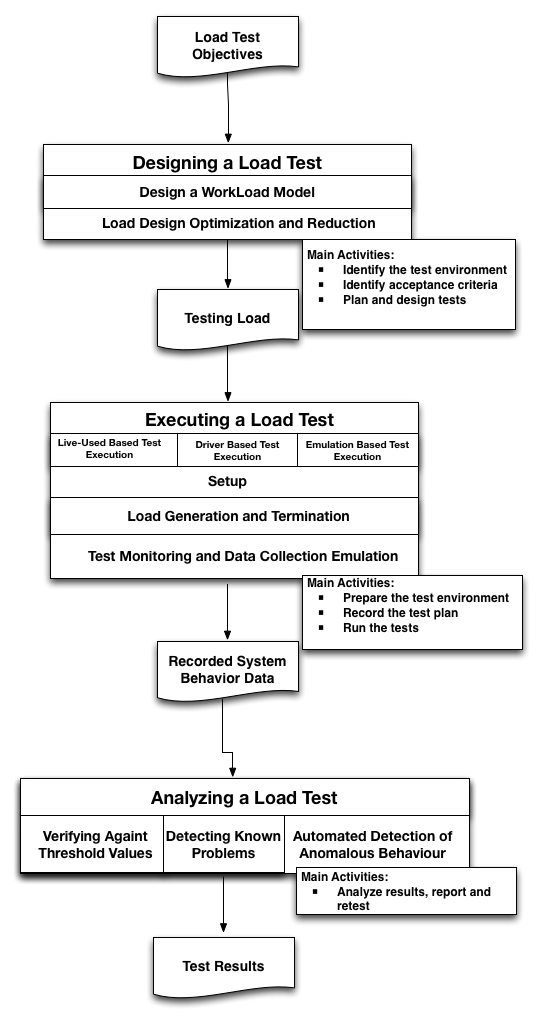
\includegraphics[width=0.5\textwidth]{./images/testprocess.png}
\caption{Load, Performance and Stress Test Process \cite{Jiang2010}\cite{Erinle2013}}
\label{fig:testprocess}
\end{figure}


The goal of the load design phase is to devise a load, which can uncover non-functional problems. Once the load is defined, the system under test executes the load and the system behavior under load is recorded. Load testing practitioners then analyze the system behavior to detect problems \cite{Jiang2010}. 

Once a proper load is designed, a load test is executed. The load test execution phase consists of the following three main aspects: (1) Setup, which includes system deployment and test execution setup; (2) Load Generation and Termination, which consists of generating the load; and (3) Test Monitoring and Data Collection, which includes recording the system behavior during execution\cite{Jiang2010}. 

The core activities in conducting an usual Load, Performance and Stress tests are \cite{Erinle2013}: 

\begin{itemize}
\item Identify the test environment: identify test and production environments and knowing the hardware, software, and network configurations helps derive an effective test plan and identify testing challenges from the outset.

\item Identify acceptance criteria: identify the response time, throughput, and resource utilization goals and constraints.

\item Plan and design tests:identify the test scenarios.In the context of testing, a scenario is a sequence of steps in an application. It can represent a use case or a business function such as searching a product catalog, adding an item to a shopping cart, or placing an order \cite{Corporation2007}.

\item Prepare the test environment: configure the test environment, tools, and resources necessary to conduct the planned test scenarios.

\item Record the test plan: record the planned test scenarios using a testing tool.

\item Run the tests: Once recorded, execute the test plans under light load and verify the correctness of the test scripts and output results.

\item Analyze results, report, and retest: examine the results of each successive run and identify areas of bottleneck that need addressing.  

\end{itemize}



\subsection{Automated Stress Test Tools}

Automated tools are needed to carry out serious load, stress, and performance testing. Sometimes, there is simply no practical way to provide reliable, repeatable performance tests without using some form of automation. The aim of any automated test tool is to simplify the testing process. Automated Test Tool  typically have the following components \cite{Molyneaux2009}:

\begin{itemize}
\item Scripting module: Enable recording of end-user activities in different middleware protocols;
\item Test management module: Allows the creation of test scenarios;
\item Load injectors: Generate the load with multiple workstations or servers;
\item Analysis module: Provides the ability to analyse the data collected by each test interation.
\end{itemize}

Apache JMeter is a free open source stress testing tool.  It has a large user base and offers lots of plugins to aid testing. JMeter is a desktop application designed to test and measure the performance and functional behavior of applications. The application it's purely Java-based and is highly extensible through a provided API (Application Programming Interface). JMeter works by acting as the client of a client/server application. JMeter allows multiple concurrent users to be simulated on the application \cite{Halili2008} \cite{Erinle2013}. 

JMeter has components organized  in a hierarchical manner. The Test Plan is the main component in a JMeter script. A typical test plan will consist of one or more Thread Groups, logic controllers, listeners, timers, assertions, and configuration elements:

\begin{itemize}
\item Thread Group: Test management module responsible to simulate the users used in a test. All elements of a test plan must be under a thread group.
\item Listeners: Analysis module responsible to provide access to the information gathered by JMeter about the test cases .
\item Samplers: Load injectors module responsible to send requests to a server, while Logical Controllers let you customize its logic.
\item Timers: allow JMeter to delay between each request.
\item Assertions: test if the application under test it is returning the correct results.
\item Configuration Elements: configure detais about the request protocol and test elements.
\end{itemize}


\subsection{Stress Test Results}

The system behavior recorded during the test execution phase needs to be analyzed to determine if there are any load-related functional or non-functional problems \cite{Jiang2010}.

There can be many formats of system behavior like resource usage data or end-to-end response time, which is recorded as response time for each individual request. These types of data need to be processed before comparing against threshold values.A proper data summarization technique is needed to describe these many data instances into one number. Some researchers advocate that the 90-percentile response time is a better measurement than the average/medium response time, as the former accounts for most of the peaks, while eliminating the outliers \cite{Jiang2010}.




\section{WorkLoad Model}

Load, performance, or stress testing projects should start with the development of a model for user workload that an application receives. This should take into consideration various performance aspects of the application and the infrastructure that a given workload will impact. A workload is a key component of such a model \cite{Molyneaux2009}.

The term workload represents the size of the demand that will be imposed on the application under test in an execution. The metric  used for measure a workload is dependent on the application domain, such as the length of the video in a transcoding application for multimedia files or the size of the input files in a file compression application \cite{Feitelson2013} \cite{Molyneaux2009} \cite{Goncalves2014}. 

Workload is also defined by the load distribution between the identified transactions at a given time. Workload helps researchers study the system behavior identified in several load models. A workload model can be designed to verify the predictability, repeatability, and scalability of a system \cite{Feitelson2013} \cite{Molyneaux2009}.


Workload modeling is the attempt to create a simple and generic model that can then be used to generate synthetic workloads. The goal is typically to be able to create workloads that can be used in performance evaluation studies. Sometimes, the synthetic workload is supposed to be similar to those that occur in practice in real systems \cite{Feitelson2013} \cite{Molyneaux2009}.

There are two kinds of workload models: descriptive and generative. The main difference between the two is that descriptive models just try to mimic the phenomena observed in the workload, whereas generative models try to emulate the process that generated the workload in the first place \cite{DiLucca2006}. 

In descriptive models, one finds different levels of abstraction on the one hand and different levels of fidelity to the original data on the other hand. The most strictly faithful models try to mimic the data directly using the statistical distribution of the data. The most common strategy used in descriptive modeling is to create a statistical model of an observed workload (Fig. \ref{fig:descriptivemodel}). This model is applied to all the workload attributes, e.g., computation, memory usage, I/O behavior, communication, etc. \cite{DiLucca2006}. Fig. \ref{fig:descriptivemodel} shows a simplified workflow of a descriptive model. The workflow has six phases. In the first phase, the user uses the system in the production environment. In the second phase, the tester collects the user's data, such as logs, clicks, and preferences, from the system. The third phase consists in developing a model designed to emulate the user's behavior. The fourth phase is made up of the execution of the test, emulation of the user's behavior, and log gathering.



\begin{figure}[!ht]
\centering
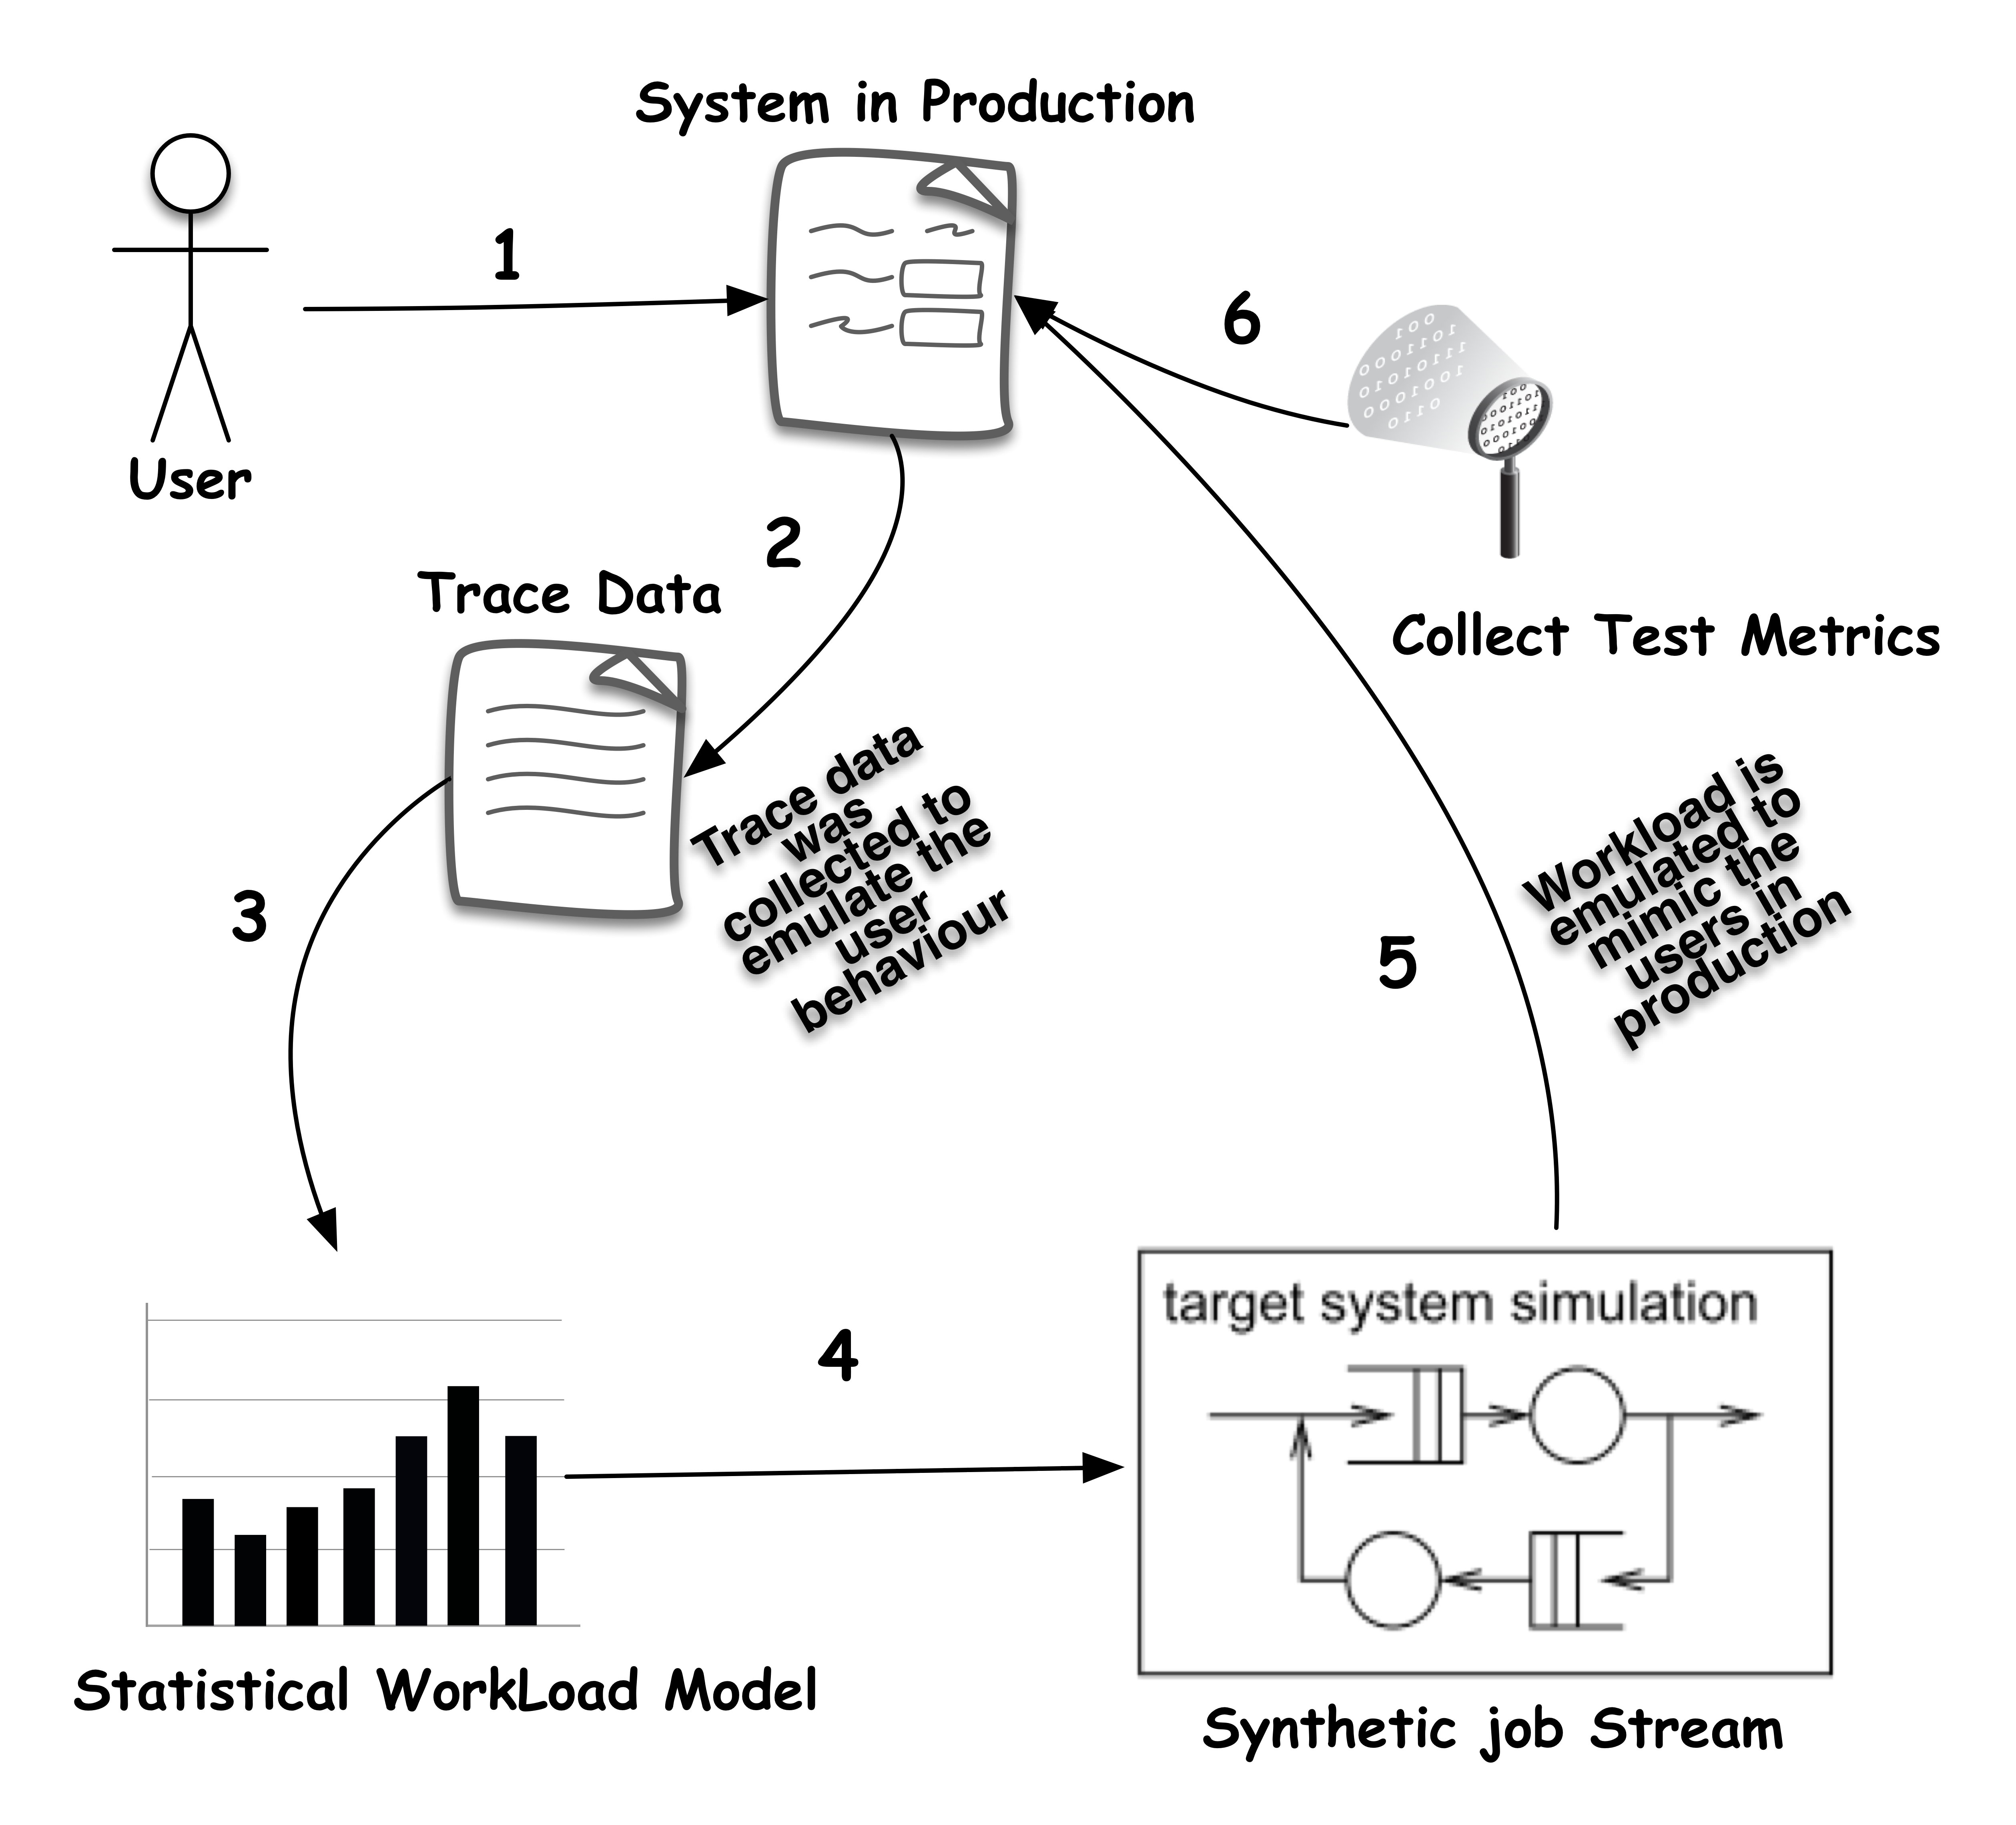
\includegraphics[width=0.4\textwidth]{./images/workloadmodel1300dpi.png}
\caption{Workload modeling based on statistical data \cite{DiLucca2006}}
\label{fig:descriptivemodel}
\end{figure}

Generative models are indirect in the sense that they do not model the statistical distributions. Instead, they describe how users will behave when they generate the workload. An important benefit of the generative approach is that it facilitates manipulations of the workload. It is often desirable to be able to change the workload conditions as part of the evaluation. Descriptive models do not offer any option regarding how to do so. With the generative models, however, we can modify the workload-generation process to fit the desired conditions \cite{DiLucca2006}. The difference between the workflows of the descriptive and the generative models is that user behavior is not collected from logs, but simulated from a model that can receive feedback from the test execution (Fig. \ref{fig:generativemodel}).

\begin{figure}[!ht]
\centering
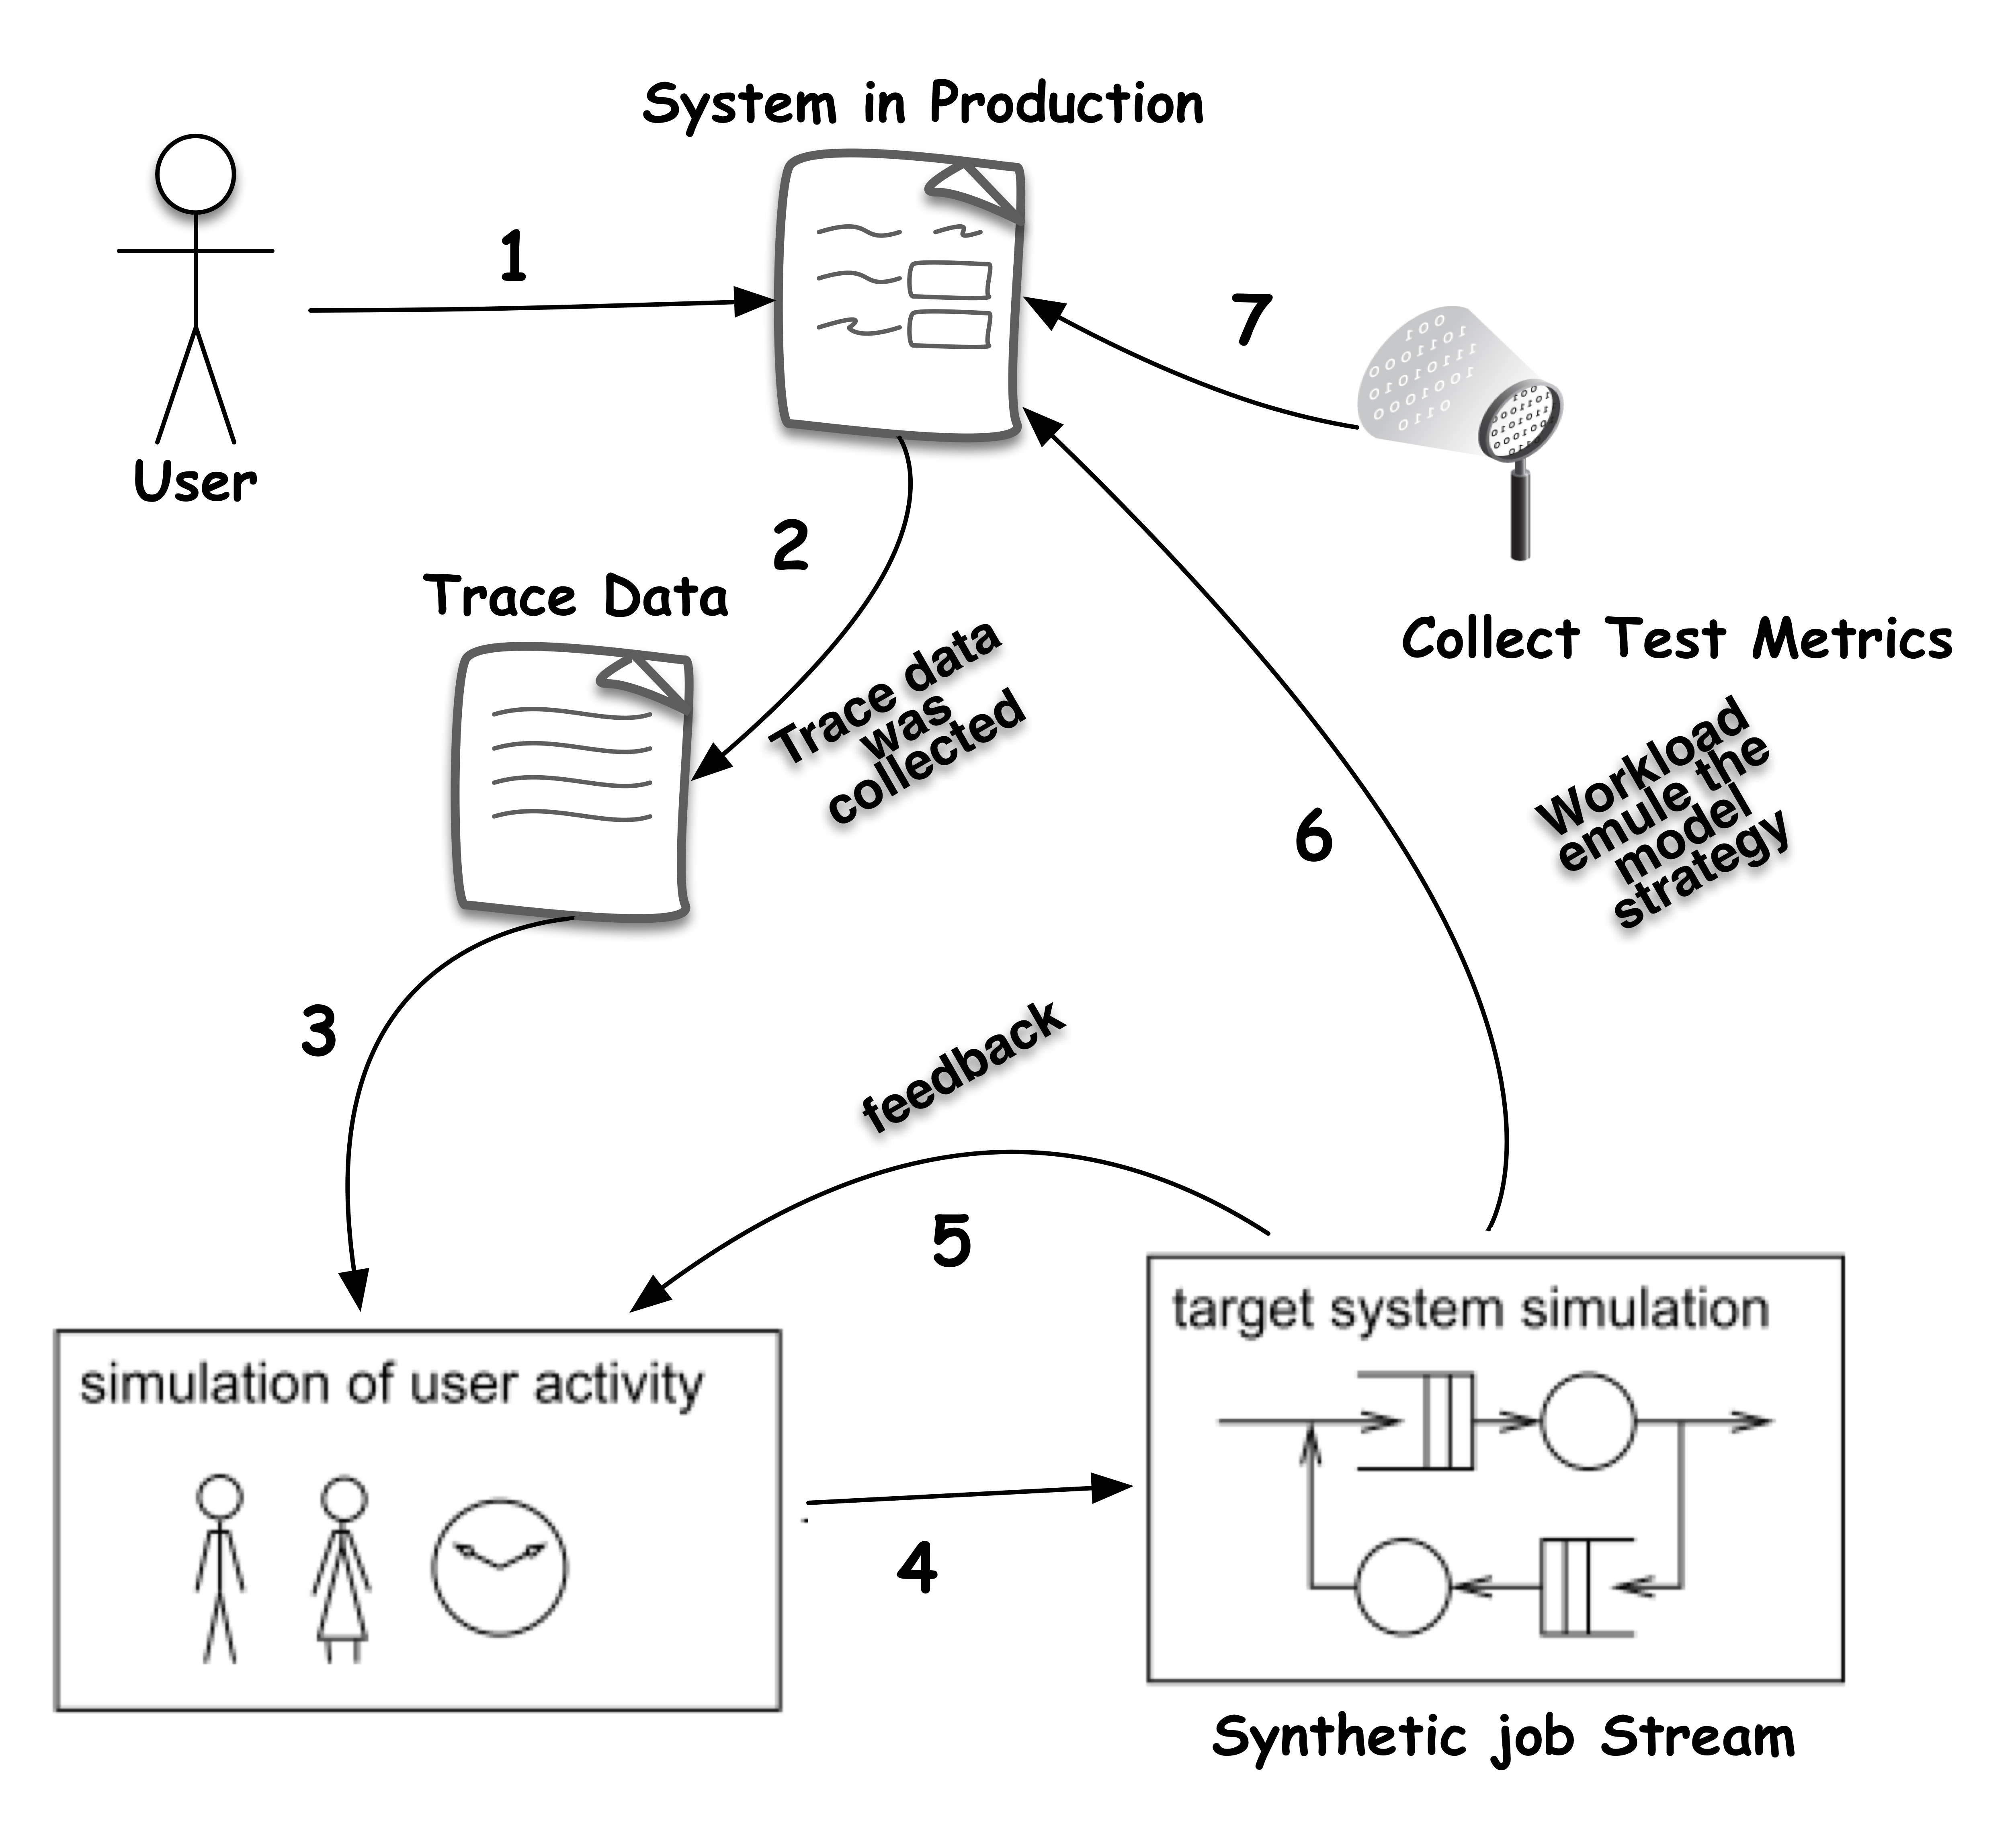
\includegraphics[width=0.4\textwidth]{./images/workloadmodel2300dpi.png}
\caption{Workload modeling based on the generative model \cite{DiLucca2006}}
\label{fig:generativemodel}
\end{figure}

Both load model have their advantages and disadvantages. In general, loads resulting from realistic-load based design techniques (Descriptive models) can be used to detect both functional and non-functional problems. However, the test durations are usually longer and the test analysis is more difficult. Loads resulting from fault-inducing load design techniques (Generative models) take less time to uncover potential functional and non-functional problems, the resulting loads usually only cover a small portion of the testing objectives \cite{Jiang2010}. The presented research work uses a generative model.



\section{Common performance application problems and performance anti-patterns}

Performance, both responsiveness and scalability, is critical to the success of today’s software systems. Many software products fail to meet their performance objectives when they are initially constructed. Performance problems share common symptoms and many performance problems described in the literature are defined by a particular set of root causes. Fig. \ref{fig:symptoms}  shows the symptoms of known performance problems \cite{Wert2013a}. 



\begin{figure}[h]
\centering
\includegraphics[width=0.7\textwidth]{./images/symptoms.png}
\caption{Symptoms of know performance problems \cite{Wert2013a}. }
\label{fig:symptoms}
\end{figure}


Symptoms combine common characteristics of a set of performance problems. Each symptom is refined by more specific performance problems that further limit the set of possible root causes. There are several anti-patterns that presents some common performance problems. Antipatterns [Brown, et al. 1998] are conceptually similar to patterns in that they document recurring solutions to common design problems. They are known as
anti-patterns because their use produces negative consequences.  Performance antipatterns document common performance mistakes made in software architectures or designs.


\subsection{Unbalanced Processing} 

Unbalanced Processing it's characterizes for one scenario where a specific class of requests generates a pattern of execution within the system that tends to overload a particular resource. In other words the overloaded resource will be executing a certain type of job very often, thus in practice damaging other classes
of jobs that will experience very long waiting times.


Unbalanced Processing occurs in three different situations. The first case that cause unbalanced processing it is when processes cannot make effective use of available processors either because processors are dedicated to other tasks or because of single-threaded code. This manifestation has available processors and we need to ensure that the software is able to use them. 


In Pipe and Filter Architectures, The throughput of the overall system is determined by the slowest filter. For example, in the travel analogy, passengers must go through several stages (or filters): first check in at the ticket counter, then pass through security, then go through the boarding process. A slow security filter could impact an entire system. 


Fig.  shows a sample of the Unbalanced Processing. 

\begin{figure}[h]
\centering
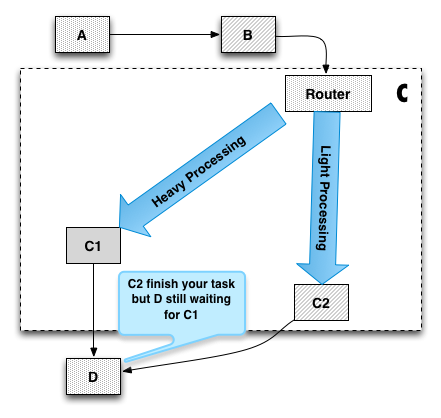
\includegraphics[width=0.7\textwidth]{./images/unbalanced.png}
\caption{Unbalanced Processing sample \cite{Wert2013a}. }
\label{fig:unbalanced}
\end{figure}



\subsection{Excessive Dynamic Allocation}

Using dynamic allocation, objects are created when they are first accessed and then destroyed when they are no longer needed. This can often be a good approach to structuring a system, providing flexibility in highly dynamic situations. Excessive Dynamic Allocation, however, addresses frequent, unnecessary creation and destruction of objects of the same class \cite{Smith2002}.



\section{Search Based Tests}

Search-based software engineering (SBSE) is the application of optimization techniques in solving software engineering problems [1,2]. The applicability of optimization techniques in solving software engineering problems is suitable as these problems frequently encounter competing constraints and require near optimal solutions \cite{Afzal2009a} \cite{Harman2015}. 


Search Based Software Testing (SBST) is the sub-area of Search Based Software Engineering concerned with software testing. Search-based software testing is the application of metaheuristic search techniques to generate software tests. SBSE uses computational search techniques to tackle software engineering problems, typified by large complex search spaces. SBSE derives test inputs for a software system with the goal of improving various criteria. The test adequacy criterion is transformed into a fitness function and a set of solutions in the search space are evaluated with respect to the fitness function using a metaheuristic search technique \cite{Afzal2009a} \cite{Aleti2016} \cite{Harman2015}.


Figure \ref{fig:sbsesbst}  shows the growth in papers published on SBST and SBSE. The data is taken from the SBSE repository (\url{http://crestweb.cs.ucl.ac.uk/resources/sbse_repository/}) [130]. 
The aim of the SBSE repository is to contain every SBSE paper. Although no repository can guarantee 100\% precision and recall, the SBSE repository has proved sufficiently usable that it has formed the basis of several other detailed analyses of the literature \cite{Harman2015}. 


\begin{figure}[h]
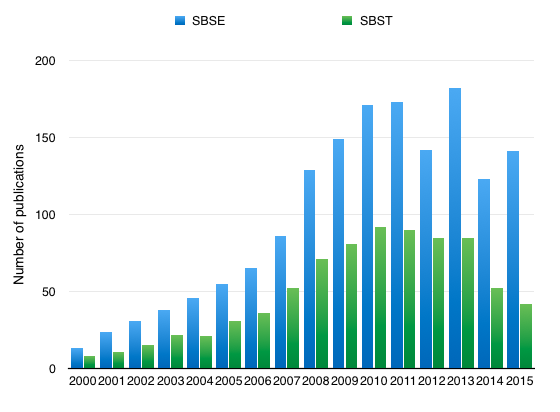
\includegraphics[width=0.5\textwidth]{./images/publications1.png}
\caption{Number of publications in SBSE and SBST by Year. Data comes from the Harman et al., Afzal et al. and the SBSE repository  \cite{Afzal2009a} \cite{Harman2015}}
\label{fig:sbsesbst}
\end{figure}


SBST has made many achievements, and demonstrated its wide applicability and increasing uptake. Nevertheless, there are pressing open problems and challenges that need more attention like to extend SBST to test non-functional properties, a topic that remains relatively under-explored, compared to structural testing. The Fig. \ref{fig:nonfunctional} shows the non-funtional SBST by year \cite{Aleti2016} \cite{Harman2015}. 

\begin{figure}[h]
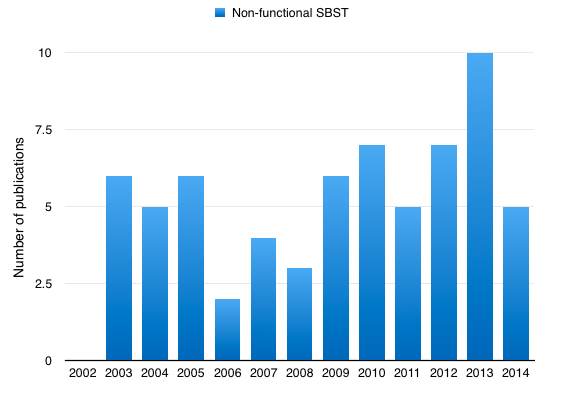
\includegraphics[width=0.5\textwidth]{./images/nonfunctional.png}
\caption{Number of publications in non-functional SBST by Year. Data comes from the Harman et al., Afzal et al. and the SBSE repository  \cite{Afzal2009a} \cite{Harman2015} }
\label{fig:nonfunctional}
\end{figure}

There are many kinds of non-functional search based tests  \cite{Afzal2009a}:

\begin{itemize}
\item Execution time: The application of evolutionary algorithms to find the best and worst case execution times (BCET, WCET).
\item Quality of service: uses metaheuristic search techniques to search violations of service level agreements (SLAs).
\item Security: apply a variety of metaheuristic search techniques  to detect security vulnerabilities like detecting buffer overflows.
\item Usability: concerned with construction of covering array which is a combinatorial object.
\item Safety: Safety testing is an important component of the testing strategy of safety critical systems where the systems are required to meet safety constraints.
\end{itemize}

A variety of metaheuristic search techniques are found to be applicable for non-functional testing including simulated annealing, tabu search, genetic algorithms, ant colony methods, grammatical evolution, genetic programming and swarm intelligence methods.

\section{Metaheuristics}

In the computer science, the term metaheuristic is accepted for general techniques which are not specific to a particular problem. A metaheuristic is formally defined as an iterative generation process which guides a subordinate heuristic by combining intelligently different concepts for exploring and exploiting the search space \cite{raidl2010metaheuristic}. 

Metaheuristics are strategies that guide the search process to efficiently explore the search space in order to find optimal solutions. Metaheuristic algorithms are approximate and usually non-deterministic and sometimes incorporate mechanisms to avoid getting trapped in confined areas of the search space. There are different ways to classify and describe metaheuristic algorithm \cite{Blum2003}:

\begin{itemize}
\item Nature-inspired vs. non-nature inspired. There are nature-inspired algorithms, like Genetic Algorithms and Ant Algorithms, and non nature-inspired ones such as Tabu Search and Iterated Local Search. 

\item Population-based vs. single point search. Algorithms working on single solutions are called trajectory methods, like Tabu Search, Iterated Local Search and Variable Neighborhood Search. They all share the property of describing a trajectory in the search space during the search process. Population-based metaheuristics perform search processes which describe the evolution of a set of points in the search space.

\item One vs. various neighborhood structures. Most metaheuristic algorithms work on one single neighborhood structure. In other words, the fitness landscape topology does not change in the course of the algorithm. Other metaheuristics, such as Variable Neighborhood Search (VNS), use a set of neighborhood structures which gives the possibility to diversify the search by swapping between different fitness
landscapes.


\end{itemize}

Trajectory methods are characterized by a trajectory in the search space. Two common trajectory methods are Simulated Annealing and Tabu Search.

Simulated Annealing (SA) is a randomized algorithm that tries to avoid being trapped in local optimum solution by assigning probabilities to deteriorating moves. The SA procedure is inspired from the annealing process of solids. SA is based on a physical
process in metallurgy discipline or solid matter physics. Annealing is the process of obtaining low energy states of a solid in heat treatment \cite{Jaziri2008}. 

The algorithmic framework of SA is described in Alg. \ref{sa}.  The algorithm starts by generating an initial solution in function \textit{GenerateInitialSolution()}. The initial temperature value is determined in function \textit{SetInitialTemperature()} such that the probability for an uphill move is quite high at the start of the algorithm. At each iteration a solution $\mbox{s}_1$ is randomly chosen in function \textit{PickNeighborAtRandom(N(s))}. If \textit{$\mbox{s}_1$} is better than \textit{s}, then \textit{$\mbox{s}_1$} is accepted as new current solution. Else, if the move from \textit{s} to \textit{$\mbox{s}_1$} is an uphill move, \textit{$\mbox{s}_1$}  is accepted with a probability which is a function of a temperature parameter \textit{Tk} and \textit{s} \cite{raidl2010metaheuristic}. 

\begin{algorithm}[H]
  \caption{Simulated Annealing Algorithm}\label{sa}
  \begin{algorithmic}[1]
    
    \State $s\gets GenerateInitialSolution()$
    \State $k\gets 0 $
    \State $Tk\gets SetInitialTemperature()$
    \While{termination conditions not met }
    \State $\mbox{s}_1\gets PickNeighborAtRandom(N (s))$
    \If{$(f(\mbox{s}_1)<f(s))$}
    \State $s\gets\mbox{s}_1$
    \Else $\;$ Accept $\mbox{s}_1$ as new solution with probability p($\mbox{s}_1|$Tk,s) 
    \EndIf
    \State $K\gets K+1$
    \State $Tk\gets AdaptTemperature()$
    \EndWhile
      
  \end{algorithmic}
\end{algorithm}


Tabu Search is a metaheuristic that guides a local heuristic search procedure to explore the solution space beyond local optimal and search with short term memory to avoid cycles. Tabu Search uses a  tabu list to keep track of the last  moves, and don’t allow going back to these \cite{Glover1986}.

The algorithmic framework of Tabu Search is described in Alg. \ref{tsa}.  The algorithm starts by generating an initial solution in function \textit{GenerateInitialSolution()} and the tabu lists are initialized as empty lists in function \textit{InitializeTabuLists($\mbox{TL}_1$,...,$\mbox{TL}_r$)}. For performing a move, the algorithm first determines those solutions from the neighborhood \textit{N(s)} of the current solution \textit{s} that contain solution features currently to be found in the tabu lists. They are excluded from the neighborhood, resulting in a restricted set of neighbors \textit{$\mbox{N}_a(s)$}. At each iteration the best solution \textit{$\mbox{s}_1$} from \textit{$\mbox{N}_a(s)$} is chosen as the new current solution. Furthermore, in procedure \textit{UpdateTabuLists($\mbox{TL}_1$,...,$\mbox{TL}_r$,s,$\mbox{s}_1$)} the corresponding features of this solution are added to the tabu lists.


\begin{algorithm}[H]
  \caption{Tabu Search Algorithm}\label{tsa}
  \begin{algorithmic}[2]
    
    \State $s\gets GenerateInitialSolution()$
    \State InitializeTabuLists($\mbox{TL}_1$,...,$\mbox{TL}_r$)
    \While{termination conditions not met }
    \State $\mbox{N}_a(s)\gets$ $\{\mbox{s}_1 \in N(s) |\mbox{s}_1$ does not violate a tabu condition, or it satisfies at least one aspiration condition $\}$ 
    \State $\mbox{s}_1\gets argmin\{f(\mbox{s}_2)|\mbox{s}_2 \in \mbox{N}_a(s) \}$
    \State UpdateTabuLists($\mbox{TL}_1$,...,$\mbox{TL}_r$,s,$\mbox{s}_1$)
    \State $s\gets \mbox{s}_1$
    \EndWhile
      
  \end{algorithmic}
\end{algorithm}

Population-based metaheuristics (P-metaheuristics) could be viewed as an iterative improvement in a population of solutions. First, the population is initialized. Then, a new population of solutions is generated. Finally, this new population is integrated into the current one using some selection procedures. The search process is stopped when a stopping criterion is satisfied. Algorithms such as Genetic algorithms (GA), scatter search (SS), estimation of distribution algorithms (EDAs), particle swarm optimization (PSO), bee colony (BC), and artificial immune systems (AISs) belong to this class of metaheuristics \cite{talbi2009metaheuristics}. 

Algorithm \ref{gna} shows the basic structure of GA algorithms. In this algorithm, P denotes the population of individuals. A population of offspring is generated by the application of recombination and mutation operators and the individuals for the next population are selected from the union of the old population and the offspring population \cite{raidl2010metaheuristic}.


\begin{algorithm}[H]
  \caption{Genetic Algorithm}\label{gna}
  \begin{algorithmic}[3]
    
    \State $s\gets GenerateInitialSolution()$
    \State Evaluate(P)
    \While{termination conditions not met }
    \State $\mbox{P}_1\gets$ $Recombine(P)$
    \State $\mbox{P}_2\gets$ $Mutate(\mbox{P}_1)$ 
    \State $Evaluate(\mbox{P}_2)$
    \State $P\gets Select(\mbox{P}_2,P)$
    \EndWhile
      
  \end{algorithmic}
\end{algorithm}




The Fig. presents the main architecture of the Testbed solution proposed 

\begin{figure}[H]
\centering
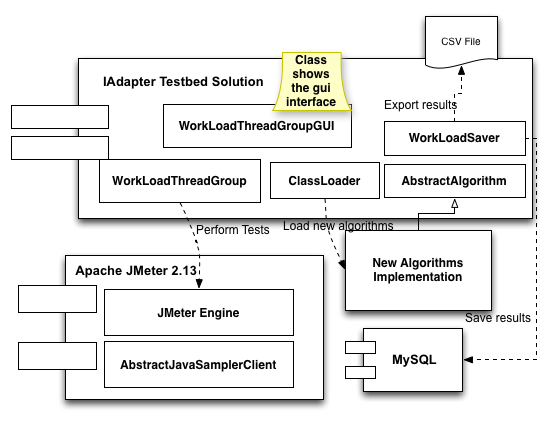
\includegraphics[width=0.8\textwidth]{./images/mainarchitect.png}
\caption{Response time results to the first battery of test.}
\label{fig:responsetimetest1}
\end{figure}

\section{Developing new algorithms to the Test Bed Solution}

To implement a new algorithm to the test bed solution it is necessary extends the class AbstractAlgorithm.

\lstdefinestyle{outline}{
		language=Java,
         basicstyle=\scriptsize\ttfamily,
         numberstyle=\tiny,
         numbersep=5pt,
         tabsize=2,
         extendedchars=true,
         breaklines=true,
         keywordstyle=\color{black}\bf,
         frame=b,  % <<<<<<<<<<<<<<<<<<<<<<<<<<
         stringstyle=\color{green!40!black}\ttfamily,
         showspaces=false,
         showtabs=false,
         numbers=left,
         xleftmargin=17pt,
         framexleftmargin=17pt,
         framextopmargin=1pt, % <<<<<<<<<<<<<<<<<<<<<<
         showstringspaces=false,
         %backgroundcolor=\color[RGB]{200,200,200},
         belowcaptionskip=0pt
}


\begin{lstlisting}[style=outline,caption={Emulated Scenario 1},label=scenario1]
public abstract class AbstractAlgorithm {
	private String methodName;
	public String getMethodName() {
		return methodName;
			}

	public void setMethodName(String methodName) {
		this.methodName = methodName;
	}

	public abstract List<WorkLoad> strategy(List<WorkLoad> list, int populationSize, List<String> testCases, int generation,
			int maxUsers, String testPlan, int mutantProbability, int bestIndividuals, boolean collaborative,
			ListedHashTree script,int maxResponseTime);
			
}
\end{lstlisting}




\section{Load Test and Experiments}

The IAdapter Test Bed Tool was validated with one  load test and 2 experiments. 

\subsection{Load Test}

The test was performed using the Apache JMeter tool to simulate the proper load to each of test scenarios prepared by the emulator. The scenarios tests 3 sample features (A,B and C functionalities). The first scenario applies successful outcomes to situations with 10 to 15 concurrent users testing A and B functionalities (Listing \ref{scenario1}) . This scenario emulated a response time according to the function $f(x)=100*numberOfThreads+1000$. 


\begin{lstlisting}[style=outline,caption={Emulated Scenario 1},label=scenario1]
if (WorkLoadThreadGroup.getScenariosSimulation().contains(a) && WorkLoadThreadGroup.getScenariosSimulation().contains(c) && numberOfThreads > 10 && numberOfThreads < 15) {
    try {
					Thread.sleep(100*numberOfThreads)+1000;
				} catch (InterruptedException e) {
					e.printStackTrace();	
				}
				sampleResult.setResponseCode("200");
				sampleResult.setSuccessful(true); }
\end{lstlisting}

The second scenario applies fail of kind JDBC Exception and 500 response code to  outcomes  with 15 to 25 concurrent users testing A and B functionalities (Listing \ref{scenario2}).  This scenario emulated a response time according to the function $f(x)=200*numberOfThreads+1000$. 

\begin{lstlisting}[style=outline,caption={Emulated Scenario 2},label=scenario2]
if (WorkLoadThreadGroup.getScenariosSimulation().contains(a) && WorkLoadThreadGroup.getScenariosSimulation().contains(c) && numberOfThreads > 15 && numberOfThreads < 25) {
    try {
					Thread.sleep(200*numberOfThreads)+1000;
				} catch (InterruptedException e) {
					e.printStackTrace();	
				}
        sampleResult.setResponseCode("500");
        sampleResult.setResponseMessage("Error on server . JDBC problem ");
        sampleResult.setSuccessful(false); }
\end{lstlisting}

The third scenario applies fail of 404 response code to  outcomes  with 15 to 25 concurrent users testing A and B functionalities (Listing \ref{scenario3}).  This scenario emulated a response time according to the function $f(x)=500*numberOfThreads+1000$. 

\begin{lstlisting}[style=outline,caption={Emulated Scenario 3},label=scenario3]
if (WorkLoadThreadGroup.getScenariosSimulation().contains(a) && WorkLoadThreadGroup.getScenariosSimulation().contains(c) && numberOfThreads > 25) {
    try {
					Thread.sleep(500*numberOfThreads)+1000;
				} catch (InterruptedException e) {
					e.printStackTrace();	
				}
        sampleResult.setResponseCode("404");
        sampleResult.setResponseMessage("Not found. ");
        sampleResult.setSuccessful(false); }
\end{lstlisting}

The fourth scenario applies fail of kind Security Error and 403 response code to  outcomes  with 10 to 15 concurrent users testing only the C functionaly (Listing \ref{scenario4}).  This scenario emulated a response time according to the function $f(x)=50*numberOfThreads+1000$. 

\begin{lstlisting}[style=outline,caption={Emulated Scenario 4},label=scenario4]
if (WorkLoadThreadGroup.getScenariosSimulation().contains(c) && (!WorkLoadThreadGroup.getScenariosSimulation().contains(a))&& (!WorkLoadThreadGroup.getScenariosSimulation().contains(b)) && numberOfThreads > 10 && numberOfThreads < 15) {
    try {
					Thread.sleep(50*numberOfThreads)+1000;
				} catch (InterruptedException e) {
					e.printStackTrace();	
				}
        sampleResult.setResponseCode("403");
        sampleResult.setResponseMessage("Security Erro.");
        sampleResult.setSuccessful(false); }
\end{lstlisting}

The success of the tests depends of the response time obtained by  the four scenarios:

\begin{itemize}
\item 2200 miliseconds to the scenario 1: $f(12)=100*(12)+1000$;
\item 4200 miliseconds to the scenario 2: $f(16)=200*(16)+1000$;
\item 14000 miliseconds to the scenario 3: $f(26)=500*(26)+1000$;
\item 1600 miliseconds to the scenario 4:
$f(12)=50*(12)+1000$;
\end{itemize}

The Fig. \ref{fig:responsetimetest1} shows the response time results for the first battery of test.

\begin{figure}[H]
\centering
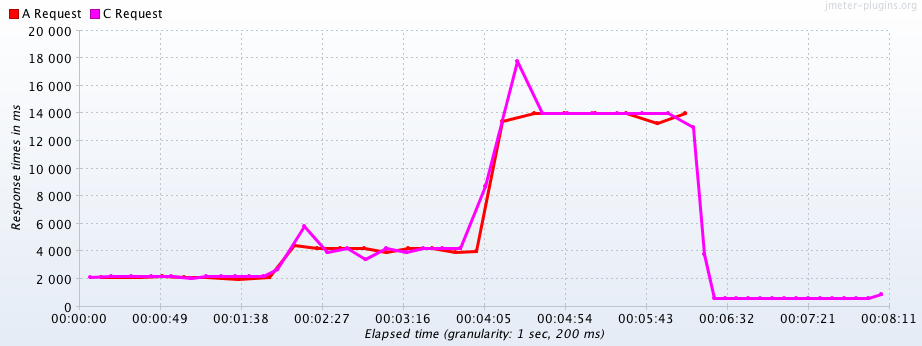
\includegraphics[width=1\textwidth]{./images/responsetimetest1.png}
\caption{Response time results to the first battery of test.}
\label{fig:responsetimetest1}
\end{figure}

We can note that in the first two minutes of testing, the response time emulated by the scenarios was 2200 milliseconds.

\subsection{First Experiment}

The first experiment was to use four metaheuristics to find the four emulated points of failure in the load test presented in the previous subsection. The first experiment was performed in 10 generations. The Fig. \ref{fig:responsetimeexperiment1} shows the response time by users. The experiment testified the correct functioning of tests that performs  scenarios 1, 2 and 3 with simultaneous users.

\begin{figure}[H]
\centering
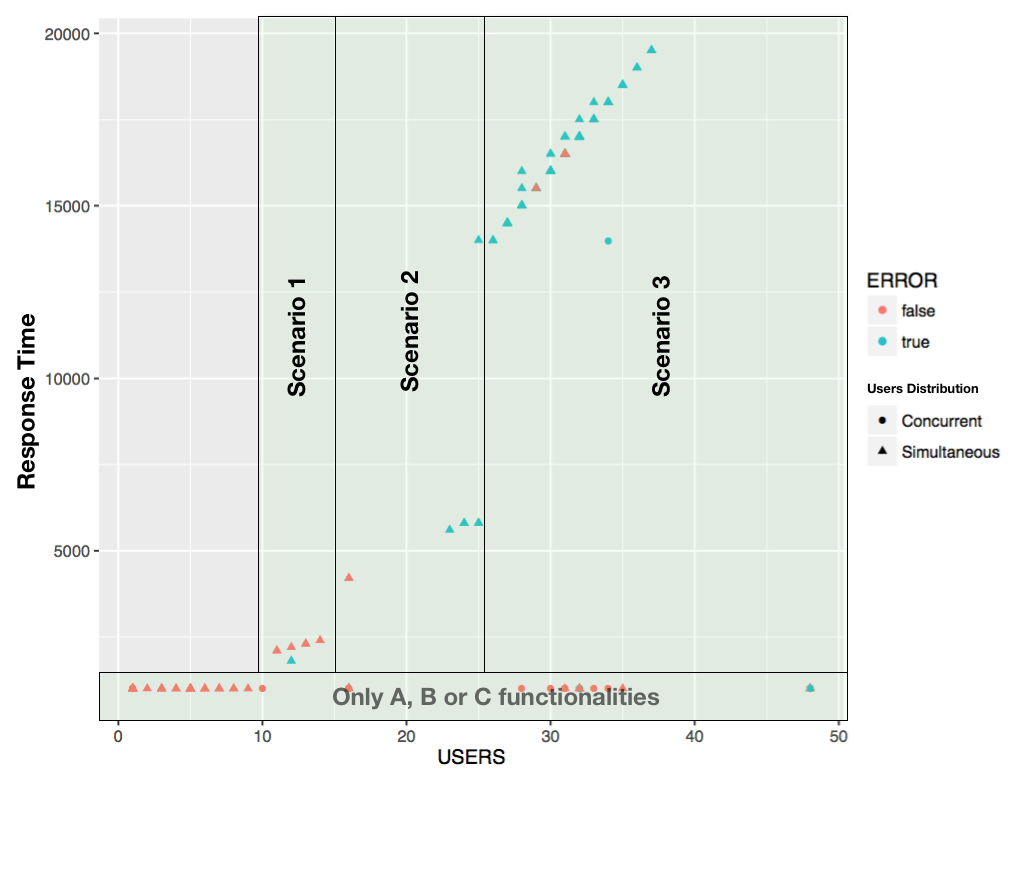
\includegraphics[width=1\textwidth]{./images/experiment1responsetime.png}
\caption{IAdapter architecture}
\label{fig:responsetimeexperiment1}
\end{figure}

The Fig. \ref{fig:totalerrorexperiment1} shows the number of errors by users. The experiment testified the correct functioning of tests that performs  scenarios 2 and 3 with simultaneous users. Some tests was applied with concurrent users. Scenario 1 does not emulated any error. The algorithms in the first experiment does not generate any individual to test the scenario 4. 

\begin{figure}[H]
\centering
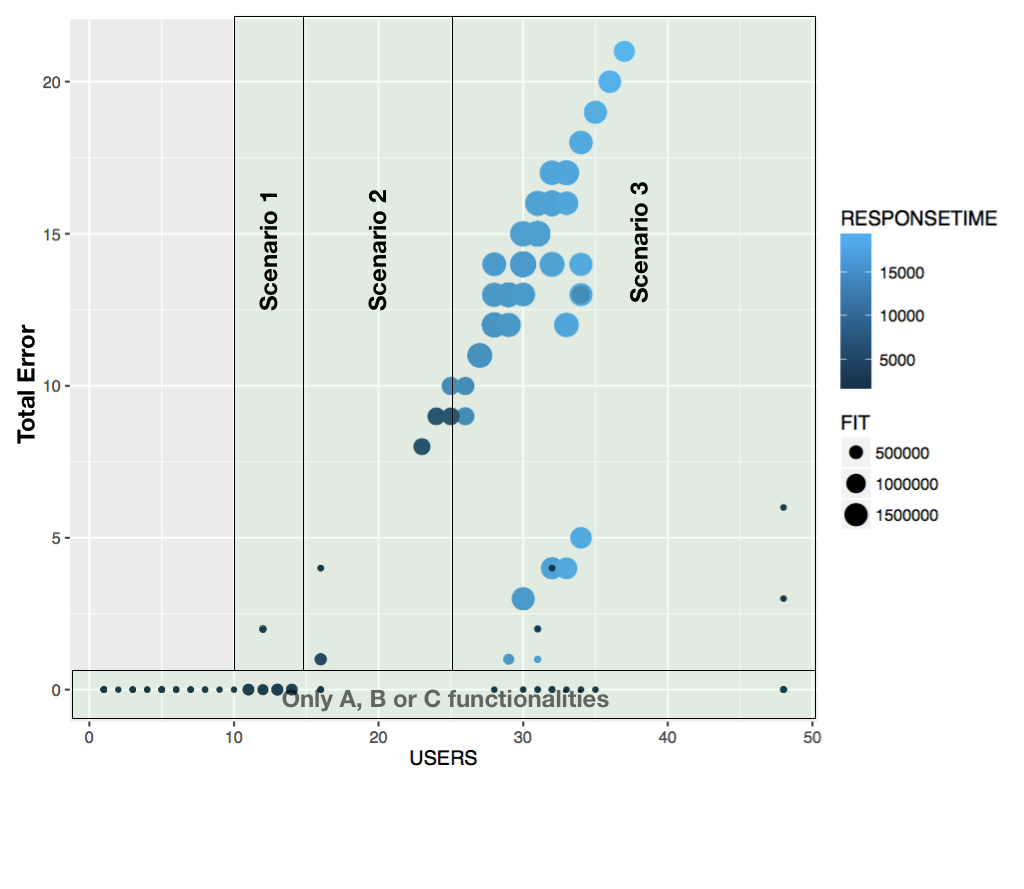
\includegraphics[width=0.8\textwidth]{./images/experiment1error.png}
\caption{Total error by users}
\label{fig:totalerrorexperiment1}
\end{figure}

The Fig. \ref{fig:fitvaluebygenerationexperiment1} shows the fit average value by generation.

\begin{figure}[H]
\centering
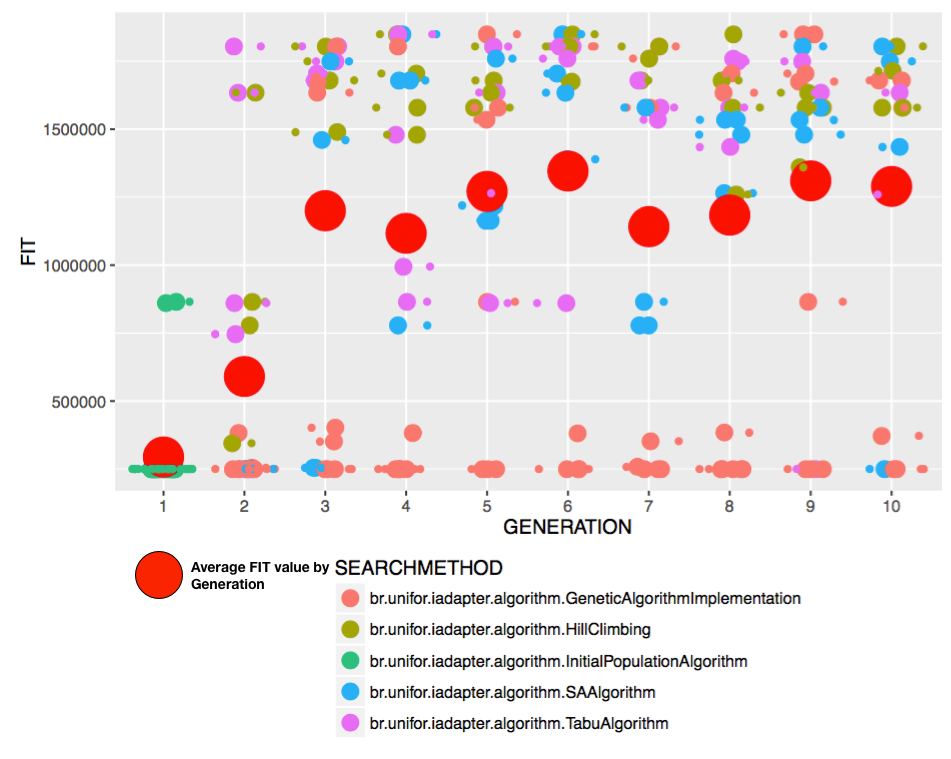
\includegraphics[width=0.8\textwidth]{./images/experiment1fitvaluebygeneration.png}
\caption{Total error by users}
\label{fig:fitvaluebygenerationexperiment1}
\end{figure}


\begin{figure}[H]
\centering
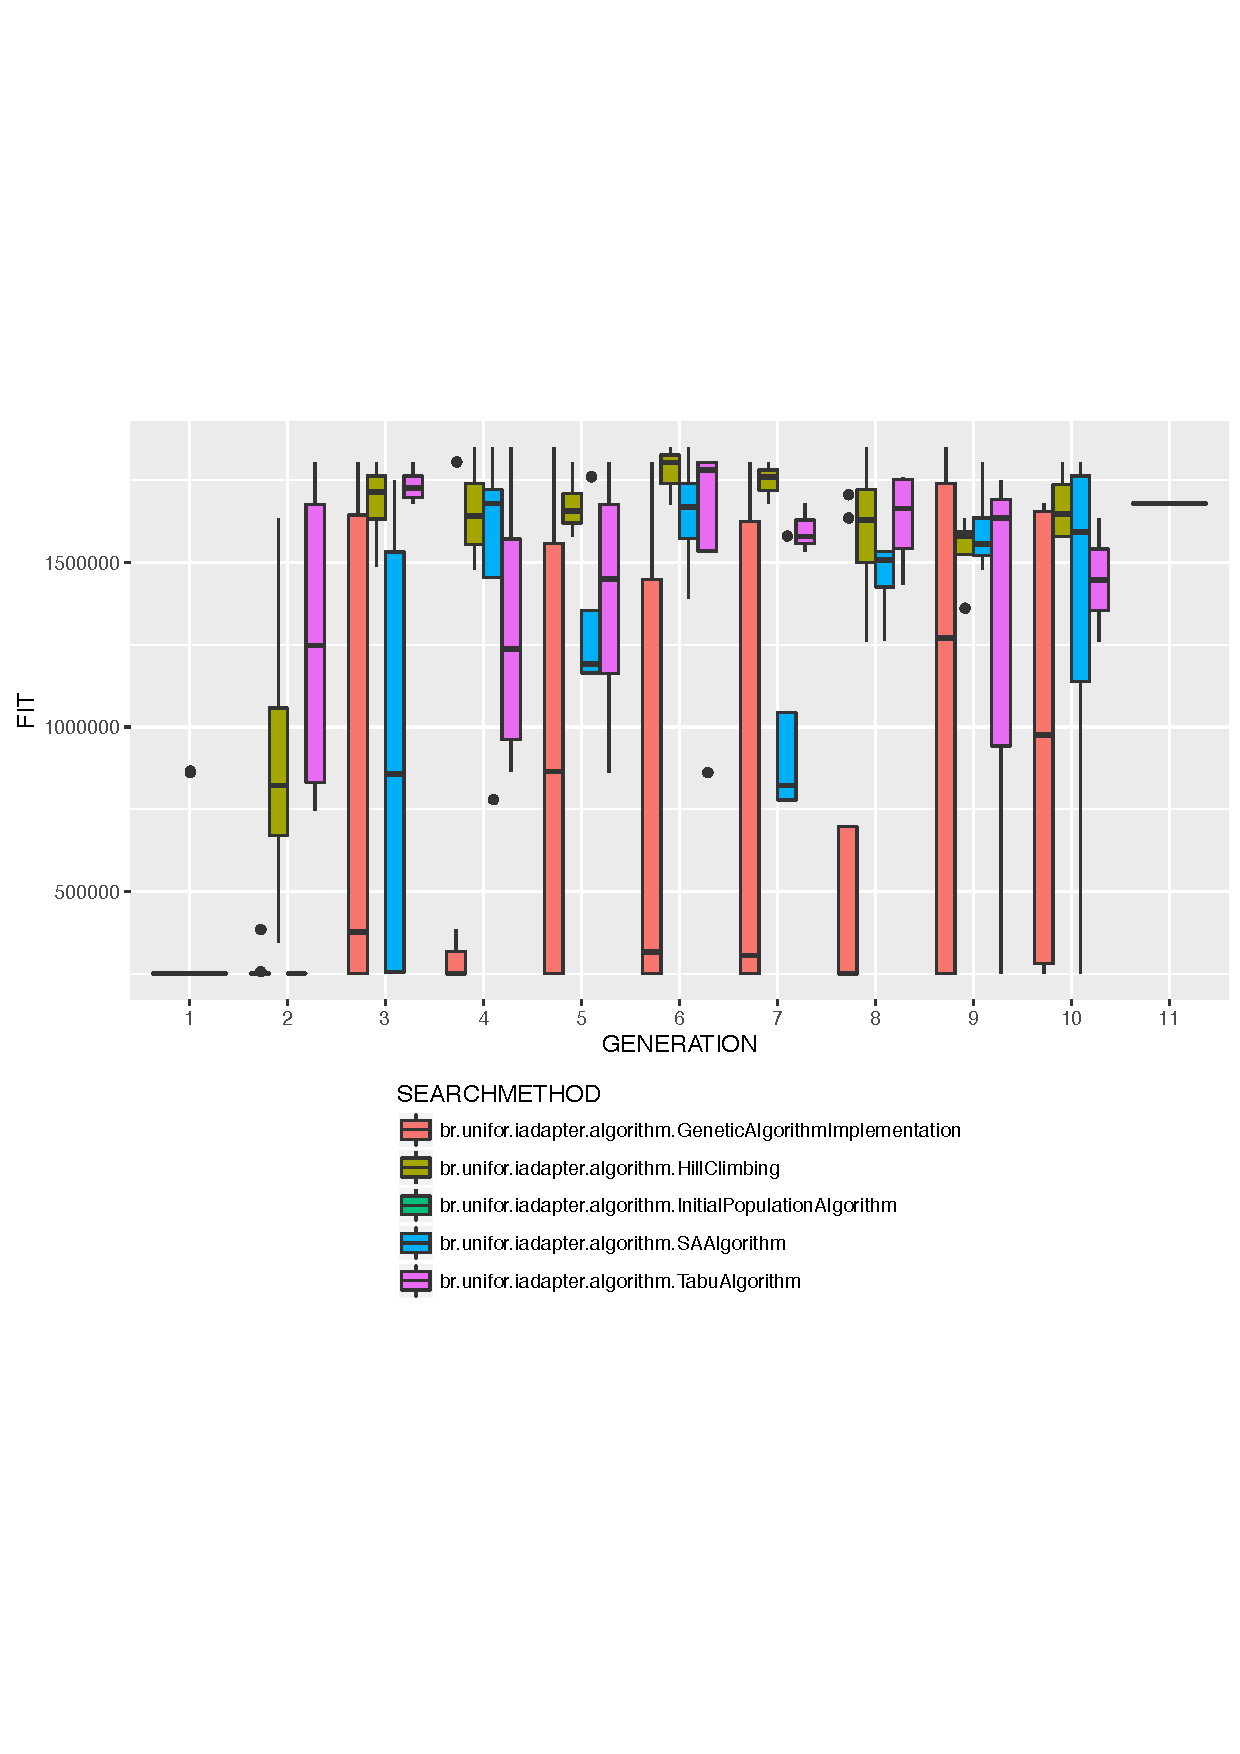
\includegraphics[width=1\textwidth]{./images/experiment1algorithms.pdf}
\caption{Total error by users}
\label{fig:fitvaluebygenerationexperiment1}
\end{figure}

\section*{References}

\bibliography{mybibfile}

\end{document}